\documentclass[../../master_thesis_np.tex]{subfiles}
\graphicspath{{./imgs/}}

\begin{document}
\chapter{Machine Learning Analysis}
\todo{machine learning analysis è molto generico... cerca un altro titolo}    

The objective of this part of the work is to build a tool to infer the interaction potential between active particles starting from the {history}\todo{serve davvero la storia?} of the positions and velocities of an ensemble of active particles.
\todo{perché vuoi fare questo? spiega}
\todo{perché il machine learning? spiega}
\todo{quali sono le difficoltà? (es. problemi con architettura standard delle reti vs. caso specifico particelle) spiega}
As explained in section \ref{literature}, one could use as input some global attribute of the system, such as the radial distribution function, but, as showed by \citeauthor{bag_interaction_2021}, this approach does not work well in out-of-equilibrium cases where an active velocity is present.
\todo{questo risolve il problema dell'architettura... ma perché non funziona? spiega meglio}

\section{Methods}
The tool we propose is based on a Graph Neural Network (GNN) that takes as input the positions and orientations of a set of active particles and tries to predict the resulting velocities.
Here, we tried to replicate the approach used by \citeauthor{ruiz-garcia_discovering_2024}, where a vector of positions and orientations of a set of active particles is given as input to a Graph Neural Network which tries to predict resulting velocities.
\todo{qual è il vantaggio di usare una GNN? spiega}
\todo{loro lo hanno usato per fare cosa? dati simulati o sperimentali? quali potenziali? spiega}
\todo{in cosa il nostro lavoro è simile? in cosa è diverso? spiega}

\subsection{The Graph Neural Network}
Our GNN is structured as explained in section \ref{literature}, namely with a node and a message function. 
Both of them have 4 layers, with 300 hidden nodes; each hidden layer has a ReLU (Rectified Linear Unit) activation function, while the output layer of each Network is a simple linear layer without any activation.
As for Figure \ref{fig:ruiz1}, the input layer of the message function is $2n_f$ dimensional, where $n_f$ is the number of single particle features, namely $x$, $y$, and $\theta$, to have information about positions and orientations of each pair of interacting agents.
Messages are aggregated using sum as an aggregation function (\verb|'add'| in PyG jargon) to respect the physics of the problem.
The node function's input dimension is $n_f + n_m$ where $n_m$ is the output dimension of the message function; this is done because the node function has the purpose of taking the aggregated message from all the senders (particle inside a threshold distance $\Gamma$) along with the single features of the receiver and trying to predict the receiver's velocity (acceleration in Newtonian dynamics).
\todo{ma uno schemino? due equazioni? spiega meglio}
\todo{approfondisci questo discorso velocità/accelerazione...}	

Here it is important to note that the history\todo{vedi commento sopra} is not relevant: the network just takes one instant at a time and predicts instantaneous velocities starting from positions and orientations, without knowing what happens before or after.
Instantaneous velocities are computed dividing the difference of consecutive positions by the integration time interval, then they get checked for big jumps, that happen when periodic boundary condition correction take place.\todo{questo non è chiaro... spiega meglio; mi ricordo che abbiamo ragionato su come calcolare la velocità: spiega il ragionamento e perché è importante, aggiungi equazioni se necessario}

The problem of message dimension $n_m$ is tackled in section \ref{literature}. 
Here, we chose a message dimension $n_m = 2$, as reported in the reference paper \cite{ruiz-garcia_discovering_2024}.
\todo{perché 2? spiega; in realtà abbiamo provato anche altro, spiega perché alla fine abbiamo scelto 2}

\subsection{Simulations}
To understand the role of the potential's functional form in prediction results, we trained and tested the network on two different simulations, one done using a spring potential with $k_s = \SI{0.1}{\newton\per\meter}$ and $x_0 = \SI{12}{\um}$ and the other using a LJ potential with $\sigma = \SI{4}{\um}$ and $\epsilon = \SI{0.01}{\pico\joule}$.
\todo{aggiungi grafici dei potenziali/forze calcolati con questi parametri}
These potential have the difference in range: without limiting our interaction threshold radius, elastic force not only has effect at long distance but its absolute value increases\todo{l'hai limitato o no?}, while LJ is a short range potential.
We expect the network to perform worse on LJ since it has less relevant interactions to learn from.

These two potentials required different integration steps: \SI{e-3}{\second} for LJ and \SI{5e-2}{\second} for spring potential.
Both simulations were ran with a particle velocity of \SI{15}{\um \per \second}, in a \qtyproduct{100 x 100}{\um} box with \num{100} particles of \SI{2}{\um} in radius.

\section{Training and Testing}

We let the two systems evolve for a total simulated time of \SI{1000}{\second}, then instantaneous velocities were computed and finally a sample of \num{1000} equally spaced snapshots was taken from each simulation.
We divided these snapshots in \num{750} for training and \num{250} for testing.
The network was trained and tested on each simulation's data separately to have preliminary results.
We tried the same procedure explained in \cite{ruiz-garcia_discovering_2024}, where two particles are considered as linked in the graph if their distance is less than some threshold, and then increasing the threshold in subsequent training loops.
In our case, after learning with the first threshold distance, loss does not decrease and test results do not improve, so what follows refers to a threshold distance of \SI{20}{\um}.
\todo{perché non funziona? spiega; come sono i nostri potenziali a 20um? che soglie hanno usato loro? con che potenziali? analizza criticamente}

After each epoch, the network is used to predict velocities on the test set, which contain data with the same potential used in training, saving the message function outputs.
Then, a minimization process is used to find the best linear transformation that maps message components into the known forces.
This is done to see how results change with the epochs.

\section{Results} \label{4results}
As showed in Figure \ref{fig:learning_curve}, in both cases loss decreases in the 100 epochs of training, meaning that the network is in fact learning.

\begin{figure}[b]
	\centering
	\subfloat{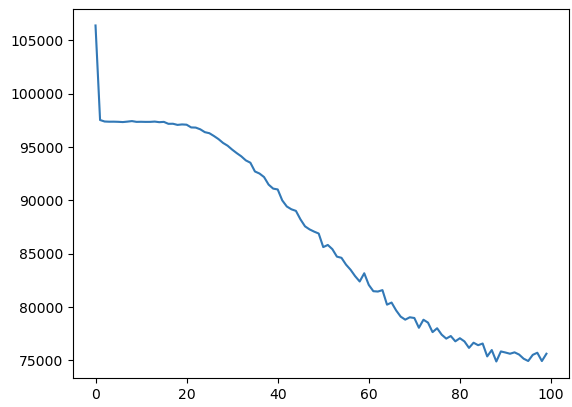
\includegraphics[width=\subfigwidth]{sp_lc.png}}
	\subfloat{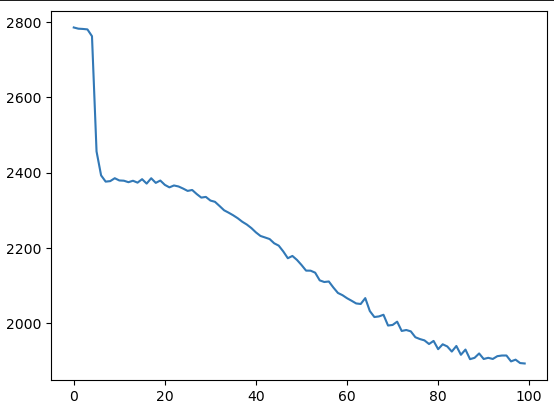
\includegraphics[width=\subfigwidth]{lj_lc.png}}
	\caption{\textbf{NOT DEFINITIVE IMAGES} Learning curve for elastic potential (left) and Lennard Jones (right). Loss is the absolute difference between predicted and ground truth velocities.}
	\label{fig:learning_curve}
\end{figure}
\todo{come è calcolata la loss? spiega; il valore assoluto è importante? spiega; se sì, uniforma gli assi y delle due figure}

Regarding the message-force plot\todo{prima introducili: a cosa servono? come li fai? equazioni}, a working network with the right linear transformation should show points on the $x = y$ line, being the message components in perfect correspondence with a rotation of the force components as \ref{fig:cranmer1} shows.
In Figure \ref{fig:lincomb} we reported the qualitatively best results, since the loss scoring in this case does not reflect a prediction quality.
\todo{perché? spiega; cosa si vede? spiega; nel paper di Ruiz-Garcia questi plot non ci sono}


\begin{figure}[tp]
	\centering
	\subfloat[][]{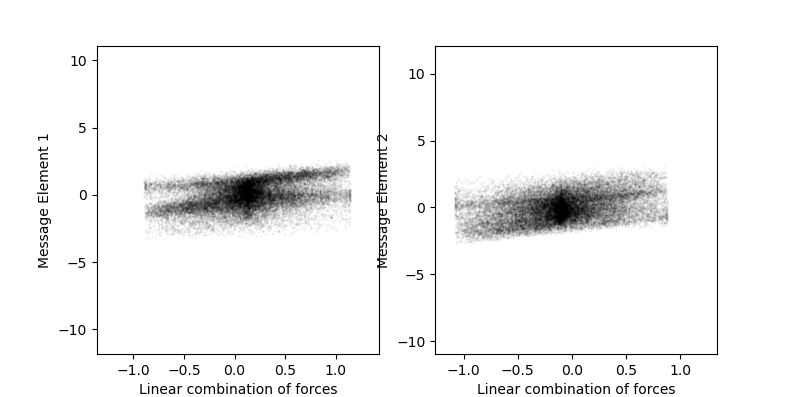
\includegraphics[width=\subfigwidth]{sp_res1.png}}
	\subfloat[][]{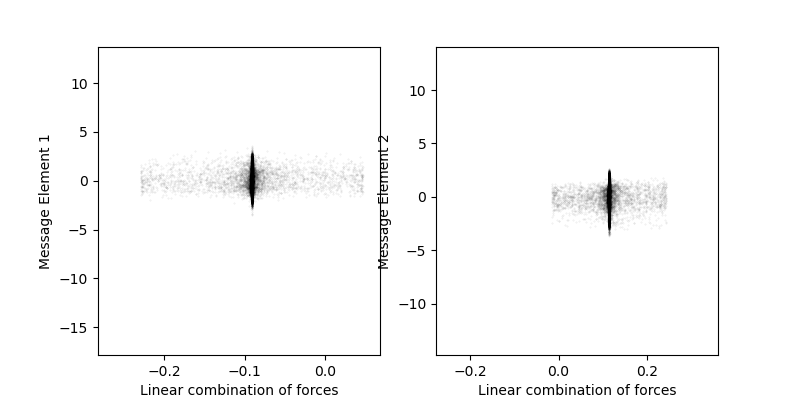
\includegraphics[width=\subfigwidth]{lj_res1.png}}
	\caption{\textbf{NOT DEFINITIVE IMAGES} Representative message-force plots of early epochs of training for spring potential (left) and Lennard Jones (right).}
	\label{fig:lincomb}
\end{figure}

As the animation in \cite{cranmer_discovering_2020} shows, as the network learns, the message-force graphs should show a better agreement between what is learned by the GNN and ground-truth.
In our case, as it is shown in fig \ref{fig:lincomb_last}, in the case of spring potential, the message-force plot has all the points on a vertical line, showing no correspondence between the learned results and ground-truth forces.
This could be caused by a tendency to overfit on the presented data, since loss is decreasing while test result are worse.

\todo{sarebbe interessante vedere dei grafici della forza vs. distanza, ma visto che non riusciamo a mappare le componenti del messaggio alle forze, potremmo dare un'occhiata ai messaggi (norma?) vs. distanza}

Anyway, it is possible to notice a difference between the two potentials\todo{in quale delle due figure?}: in the case of Lennard Jones, few points are outside the vertical line and they position in an horizontal cloud around it, while for the elastic potential most points are scattered around an horizontal cloud and a density increase can be observed in diagonal lines.\todo{nella prima figura?}

\begin{figure}[tp]
	\centering
	\subfloat[][]{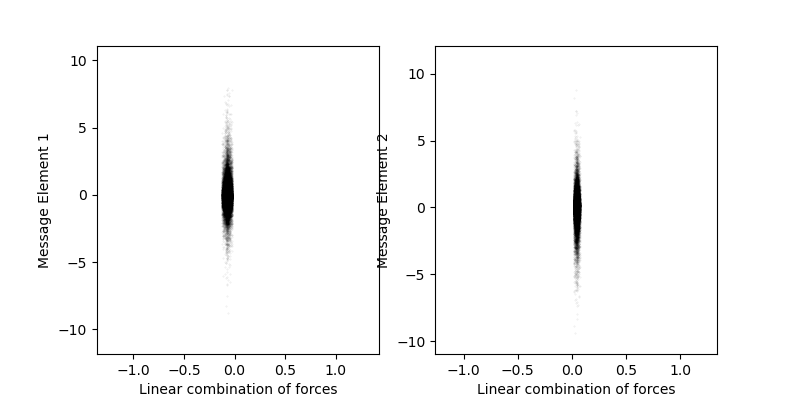
\includegraphics[width=\subfigwidth]{sp_reslast.png}}
	\subfloat[][]{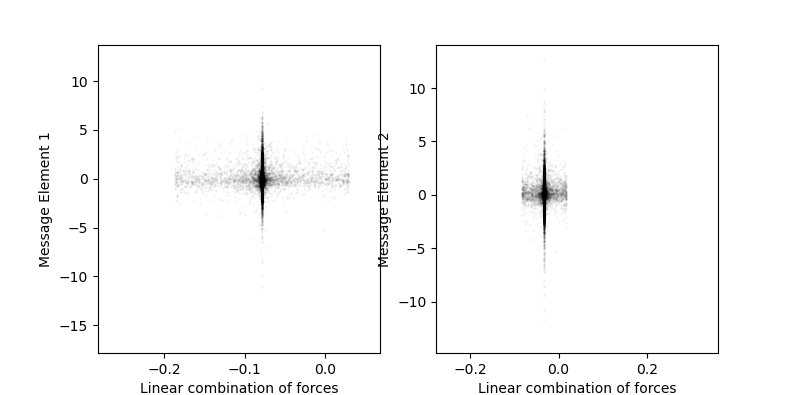
\includegraphics[width=\subfigwidth]{lj_reslast.png}}
	\caption{\textbf{NOT DEFINITIVE IMAGES} Representative message-force plots of last epoch of training for spring potential (left) and Lennard Jones (right).}
	\label{fig:lincomb_last}
\end{figure}

\todo{queste immagini sono troppo piccole}

\section{Conclusions to Chapter 4}

Here we presented the preliminary version and results of a machine learning tool that predicts forces between interacting active particles, in the spirit of the ActiveNet system developed by \citeauthor{ruiz-garcia_discovering_2024}.

As shown in section \ref{4results}, more work is needed in order to make this tool work as expected.
In particular, training for longer with more simulation snapshots is certainly needed in order to get the right accuracy.
\todo{fai un confronto critico con la sezione 3 in appendice C del loro paper}
Retraining process with increasing threshold distance must be perfected, in order to get at the same level of the reference paper.
\todo{poteva aver senso partire con soglie più basse, considerando i nosri potenziali? spiega}

After making the training process work as desired, the next step is to retrain the network with snapshots taken from simulations with different potentials, in order to increase its generalization capability.

Moreover, testing with experimental data will need some more adjustments.
In an experimental setting, defects inherited from the fabrication process like stuck particles and particle clumps can make it harder for a machine learning tool to work properly.
In the case of experimental data collected in the Microscale Robotics Lab, it is hard to measure particles' orientation, since the two hemispheres of silica Janus particles are not clearly distinguishable, though a difference in color is noticeable.
Moreover, these particles are free to rotate in three dimensions and nothing prevents them from pointing one hemisphere to the microscope objective, not showing the separation line.
\todo{cosa si può fare in assenza di informazioni sull'orientamento? spiega (ne abbiamo parlato)}

We can state that these results, though certainly not satisfying, can be a starting point to further developments of this tool, getting it to work as expected in the case of active particles like those under investigation in the host laboratory.
With the potentials inferred from experiments, we would be able to model particles in a more accurate and complete way, to simulate them and use simulated data back in a simulation-driven inference fashion.
\end{document}